

\actTitle{Worksheet 2.1A}


\noindent \textbf{Instructions:}  Work together in groups of  3 or 4 to complete the following problems.




\begin{enumerate}
\item Given $f(x)=(x+2)^2-1$.
\begin{enumerate}
\item Determine whether the graph of the parabola opens upward or
  downward.
  \sideNote{Include a brief justification.}
  \vfill
\item Identify the coordinate for the vertex. \\ [1cm]
\item Determine the $x$-intercept(s).
  \vfill
\item Determine the $y$-intercept.
  \vfill
\item Sketch the function.\\
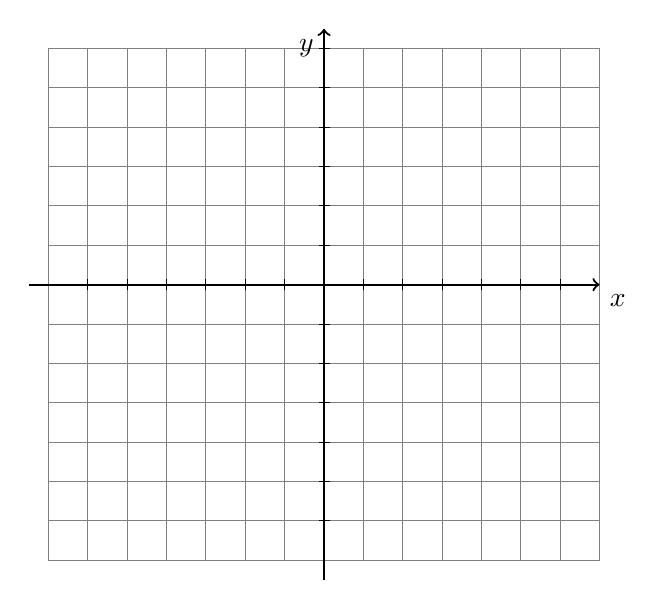
\begin{tikzpicture}[y=.5cm, x=0.5cm,font=\sffamily]
    %% ticks
    \draw[step = 1, gray] (-7,-7) grid (7,6);
    %% axis
    \draw[thick,->] (-7.5,0) -- coordinate (x axis mid) (7,0) node[anchor = north west] {$x$};
    \draw[thick,->] (0,-7.5) -- coordinate (y axis mid) (0,6.5) node[anchor = north east] {$y$};
    \foreach \y in {-6,-5,...,-1,1,2,...,6} {
      \draw (2pt, \y) -- (-2pt, \y);
    }
    \foreach \x in {-6,-5,...,-1,1,2,...,6} {
      \draw (\x,2pt) -- (\x,-2pt);
    }

\end{tikzpicture}

\item Determine the axis of symmetry.

\end{enumerate}


\clearpage

\item Find the quadratic function with the given vertex and point.
  Put your answer in standard (vertex) form.
\begin{enumerate}
\item  Vertex $(2,0)$ passing through $(1,3)$.
  \vfill
 
\item  Vertex $(-3,4)$ passing through $(0,0)$.
   \vfill
 \end{enumerate}


\item In each problem below, complete the square and then use that
  work to find the vertex of the graph of the quadratic function.
\begin{enumerate}
\item $y=x^2+4x$
  \vfill
\item  $y=-2x^2+16x-29$
  \vfill
\end{enumerate}


\clearpage 

\item Find the equation for the parabolas below.  Put your answers in standard form.
\begin{enumerate}
\item $y=$\\



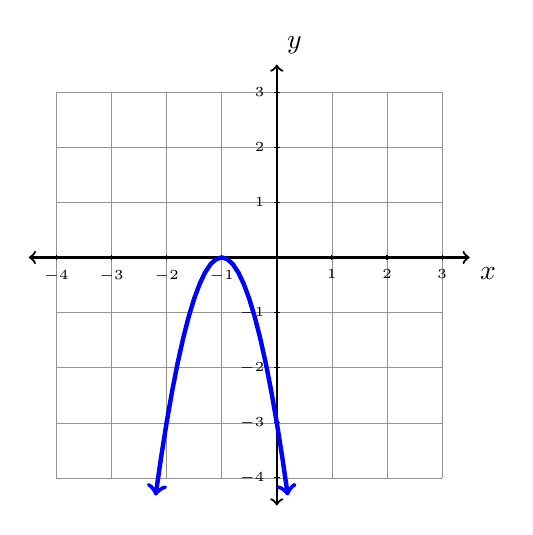
\begin{tikzpicture}[y=.7cm, x=.7cm,font=\sffamily,
	mydot/.style={
    circle,
    fill=white,
    draw,
    outer sep=0pt,
    inner sep=1.5pt
  }]
    %% Add a grid
    \draw[step = 1, gray, very thin,opacity=0.85] (-4, -4) grid (3, 3);
 	%% Draw the axes
	\draw[thick,<->] (-4.5,0) -- coordinate (x axis mid) (3.5,0) node[anchor = north west] {$x$};
    \draw[thick,<->] (0,-4.5) -- coordinate (y axis mid) (0,3.5) node[anchor = south west] {$y$};
    %% Label the y axis
    \foreach \y in {-4,...,-1,1,2,...,3} {
      \draw (1pt, \y) -- (-1pt, \y) node[anchor =  east] {\tiny$\y$};
    }
    %% Label the x axis
    \foreach \x in {-4,...,-1,1,2,...,3} {
      \draw (\x,1pt) -- (\x,-1pt) node[anchor = north] {\tiny$\x$};
    }
    %% Draw the function.
   \begin{scope}
  %       \draw[very thick,black] (-3,2) -- (1,1);
 %        \draw[very thick,black] (3.05,1.05) -- (4,3);
    %semi-circle
  %       \draw[very thick, black] (1,1) arc [radius=1, start angle=180, end angle= 5];
     %function
         \draw[ultra thick, blue, <->, domain=-2.2:.2] plot (\x, {-3*(\x+1)^2});
      
     %dots
%       \fill[blue] (2, 4) circle[radius=0.5ex];
     %  \fill[black] (1,1) circle[radius=0.5ex];
     %    \fill[black] (4,3) circle[radius=0.5ex];
     %     \draw[very thick, black] (3,1) circle[radius=0.5ex];


    \end{scope}

    %%\node[above=0.1cm] at (-2,2 )   {\nextXValue};

  \end{tikzpicture}



\item $y=$\vspace{1em}


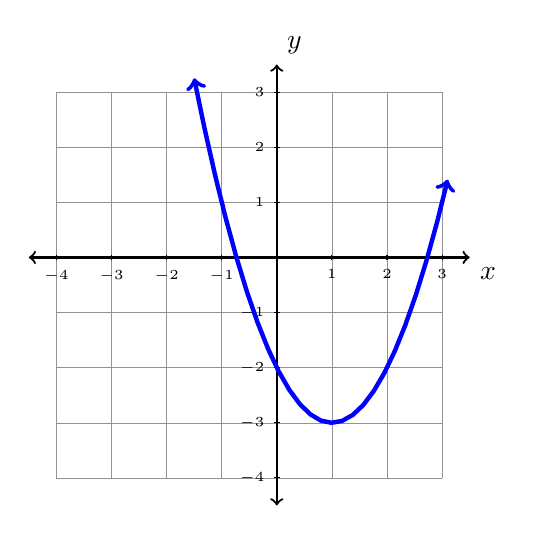
\begin{tikzpicture}[y=.7cm, x=.7cm,font=\sffamily,
	mydot/.style={
    circle,
    fill=white,
    draw,
    outer sep=0pt,
    inner sep=1.5pt
  }]
    %% Add a grid
    \draw[step = 1, gray, very thin,opacity=0.85] (-4, -4) grid (3, 3);
 	%% Draw the axes
	\draw[thick,<->] (-4.5,0) -- coordinate (x axis mid) (3.5,0) node[anchor = north west] {$x$};
    \draw[thick,<->] (0,-4.5) -- coordinate (y axis mid) (0,3.5) node[anchor = south west] {$y$};
    %% Label the y axis
    \foreach \y in {-4,...,-1,1,2,...,3} {
      \draw (1pt, \y) -- (-1pt, \y) node[anchor =  east] {\tiny$\y$};
    }
    %% Label the x axis
    \foreach \x in {-4,...,-1,1,2,...,3} {
      \draw (\x,1pt) -- (\x,-1pt) node[anchor = north] {\tiny$\x$};
    }
    %% Draw the function.
   \begin{scope}
  %       \draw[very thick,black] (-3,2) -- (1,1);
 %        \draw[very thick,black] (3.05,1.05) -- (4,3);
    %semi-circle
  %       \draw[very thick, black] (1,1) arc [radius=1, start angle=180, end angle= 5];
     %function
         \draw[ultra thick, blue, <->, domain=-1.5:3.1] plot (\x, {(\x-1)^2-3});
      
     %dots
%       \fill[blue] (2, 4) circle[radius=0.5ex];
     %  \fill[black] (1,1) circle[radius=0.5ex];
     %    \fill[black] (4,3) circle[radius=0.5ex];
     %     \draw[very thick, black] (3,1) circle[radius=0.5ex];


    \end{scope}

    %%\node[above=0.1cm] at (-2,2 )   {\nextXValue};

  \end{tikzpicture}


%\includegraphics{parabola-b}

\end{enumerate}

\vfill

\clearpage

\item Determine all values of $x$ that satisfy the following
  relationships.
\begin{enumerate}
\item $3x^2+6x=4$
\vfill
\item $x-3=\sqrt{1+2x^2}$
\vfill
\end{enumerate}

\clearpage

\item A sheet of paper will be cut in the shape of a rectangle. The
  height of the rectangle will be $x$ units, and the width of the
  rectangle will be $5-x$ units.
  \begin{enumerate}
  \item Make a rough sketch of the piece of paper and label the
    lengths of the sides.
    \vfill
  \item What are the possible range of values that $x$ could be?
    \vfill
  \item Describe what happens to the shape of the paper as the value
    of $x$ goes from its lowest possible value to its largest possible
    value.
    \vfill
  \item Determine the function of $x$ that represents the area of the
    piece of paper, and sketch the graph of the function. \\
    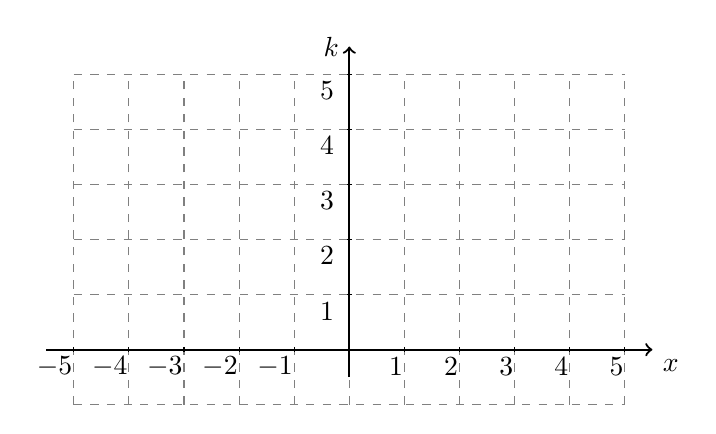
\begin{tikzpicture}[y=0.7cm, x=0.7cm,font=\sffamily]

    \begin{scope}[shift={(0,0)}]      
      %% ticks
      \draw[step = 1, gray,dashed] (-5,-1) grid (5,5);
      %% axis
      \draw[thick,->] (-5.5,0) -- coordinate (x axis mid) (5.5,0) node[anchor = north west] {$x$};
      \draw[thick,->] (0,-0.5) -- coordinate (y axis mid) (0,5.5) node[anchor = east] {$k$};
      \foreach \y in {1,2,3,4,5} {
        \draw (1pt, \y) -- (-1pt, \y) node[yshift=-6,xshift=-1,anchor=east] {$\y$};
      }
      \foreach \x in {-5,-4,-3,-2,-1,1,2,3,4,5} {
        \draw (\x,1pt) -- (\x,-1pt) node[yshift=-5,xshift=3,anchor=east] {$\x$};
      }
    \end{scope}


  \end{tikzpicture}

  \item What value of $x$ will make the area of the piece of paper as
    large as possible?
    \vfill

  \item What is the perimeter of the piece of paper given $x$?
    
  \end{enumerate}

\end{enumerate}



\hwTitle{Section 2.1A}

\begin{enumerate}
\item Find the quadratic function with the given vertex and point.
  Put your answer in standard (vertex) form.
\begin{enumerate}
\item Vertex $(0,0)$ passing through $(-2,8)$.
\item Vertex $(2,5)$ passing through $(3,-7)$.
\item Vertex $(-1,5)$ passing through $(1,4)$.
\item Vertex $(3,-2)$ passing through $(-1,0)$.
\end{enumerate}

\item In each problem below, complete the square and then use that
  work to find the vertex of the graph of the quadratic function.
\begin{enumerate}
\item $y=4x^2+8x$
\item $y=x^2-2x+2$
\item $y=6x-10-x^2$
\item  $y=-4x^2+16x-27$
\end{enumerate}

\item Find the equation for the parabolas below.  Put your answers in
  standard form.
  \begin{enumerate}
  \item $y=$\\
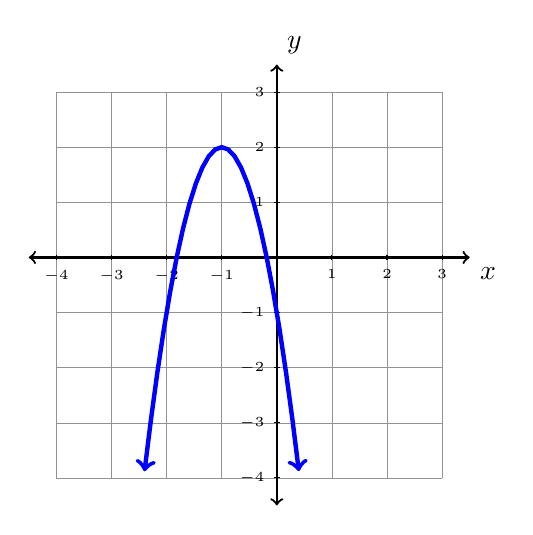
\begin{tikzpicture}[y=.7cm, x=.7cm,font=\sffamily,
	mydot/.style={
    circle,
    fill=white,
    draw,
    outer sep=0pt,
    inner sep=1.5pt
  }]
    %% Add a grid
    \draw[step = 1, gray, very thin,opacity=0.85] (-4, -4) grid (3, 3);
 	%% Draw the axes
	\draw[thick,<->] (-4.5,0) -- coordinate (x axis mid) (3.5,0) node[anchor = north west] {$x$};
    \draw[thick,<->] (0,-4.5) -- coordinate (y axis mid) (0,3.5) node[anchor = south west] {$y$};
    %% Label the y axis
    \foreach \y in {-4,...,-1,1,2,...,3} {
      \draw (1pt, \y) -- (-1pt, \y) node[anchor =  east] {\tiny$\y$};
    }
    %% Label the x axis
    \foreach \x in {-4,...,-1,1,2,...,3} {
      \draw (\x,1pt) -- (\x,-1pt) node[anchor = north] {\tiny$\x$};
    }
    %% Draw the function.
   \begin{scope}
  %       \draw[very thick,black] (-3,2) -- (1,1);
 %        \draw[very thick,black] (3.05,1.05) -- (4,3);
    %semi-circle
  %       \draw[very thick, black] (1,1) arc [radius=1, start angle=180, end angle= 5];
     %function
         \draw[ultra thick, blue, <->, domain=-2.4:.4] plot (\x, {-3*(\x+1)^2+2});
      
     %dots
%       \fill[blue] (2, 4) circle[radius=0.5ex];
     %  \fill[black] (1,1) circle[radius=0.5ex];
     %    \fill[black] (4,3) circle[radius=0.5ex];
     %     \draw[very thick, black] (3,1) circle[radius=0.5ex];


    \end{scope}

    %%\node[above=0.1cm] at (-2,2 )   {\nextXValue};

  \end{tikzpicture}


%\includegraphics{parabola-c}


    \item $y=$\\ \nopagebreak
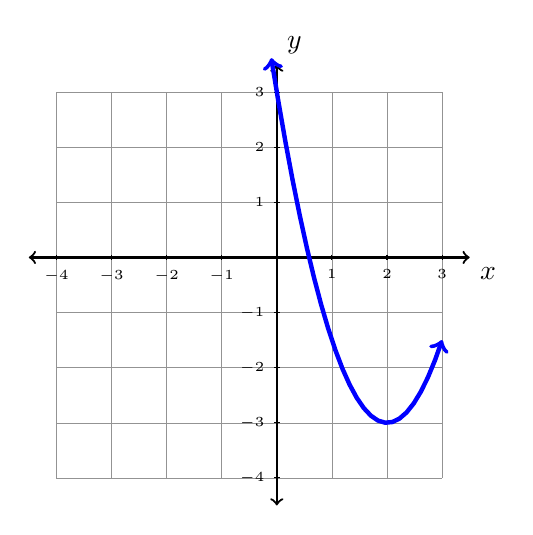
\begin{tikzpicture}[y=.7cm, x=.7cm,font=\sffamily,
	mydot/.style={
    circle,
    fill=white,
    draw,
    outer sep=0pt,
    inner sep=1.5pt
  }]
    %% Add a grid
    \draw[step = 1, gray, very thin,opacity=0.85] (-4, -4) grid (3, 3);
 	%% Draw the axes
	\draw[thick,<->] (-4.5,0) -- coordinate (x axis mid) (3.5,0) node[anchor = north west] {$x$};
    \draw[thick,<->] (0,-4.5) -- coordinate (y axis mid) (0,3.5) node[anchor = south west] {$y$};
    %% Label the y axis
    \foreach \y in {-4,...,-1,1,2,...,3} {
      \draw (1pt, \y) -- (-1pt, \y) node[anchor =  east] {\tiny$\y$};
    }
    %% Label the x axis
    \foreach \x in {-4,...,-1,1,2,...,3} {
      \draw (\x,1pt) -- (\x,-1pt) node[anchor = north] {\tiny$\x$};
    }
    %% Draw the function.
   \begin{scope}
  %       \draw[very thick,black] (-3,2) -- (1,1);
 %        \draw[very thick,black] (3.05,1.05) -- (4,3);
    %semi-circle
  %       \draw[very thick, black] (1,1) arc [radius=1, start angle=180, end angle= 5];
     %function
         \draw[ultra thick, blue, <->, domain=-0.1:3] plot (\x, {1.5*(\x-2)^2-3});
      
     %dots
%       \fill[blue] (2, 4) circle[radius=0.5ex];
     %  \fill[black] (1,1) circle[radius=0.5ex];
     %    \fill[black] (4,3) circle[radius=0.5ex];
     %     \draw[very thick, black] (3,1) circle[radius=0.5ex];


    \end{scope}

    %%\node[above=0.1cm] at (-2,2 )   {\nextXValue};

  \end{tikzpicture}


%\includegraphics{parabola-c}

\end{enumerate}

\item Solve the following equations.
\begin{enumerate}
\item $x^2-10x+8=0$.
\item $7x^2+3x=-2$.
\item $x-3=\sqrt{x+1}$.
\item $\frac{x}{x-2}=x-2$.
\end{enumerate}

\item A farmer will construct a rectangular pen. The pen will be
  divided into two equal parts by running a small fence North/South
  across the middle of the rectangle. The total width (East to West)
  of the pen will be $x$ meters, and the total height (North to South)
  will be $4-\frac{2}{3}x$ meters.
  \begin{enumerate}
  \item Make a rough sketch of the pen and labels the lengths of each
    fence.
  \item What are the possible range of values that $x$ could be?
  \item Describe what happens to the overall shape of the pen as $x$
    goes from its lowest possible value to its highest possible value.
  \item Determine the function of $x$ that represents the total area
    of the pen. Make a sketch of the graph of the function. (Label
    your axes.)
  \item What value of $x$ will result in a pen with the largest
    possible total area?
  \item What is the total length of the fencing used in the pen given
    $x$?
  \end{enumerate}


\item A farmer will construct a rectangular pen. The pen will be
  divided into three equal parts by running two small fences
  North/South across the middle of the rectangle. The total width
  (East to West) of the pen will be $x$ meters, and the total height
  (North to South) will be $9-\frac{1}{2}x$ meters. The cost of
  fencing is eight dollars per meter.
  \begin{enumerate}
  \item Make a rough sketch of the pen and labels the lengths of each
    fence.
  \item What are the possible range of values that $x$ could be?
  \item Describe what happens to the overall shape of the pen as $x$
    goes from its lowest possible value to its highest possible value.
  \item Determine the function of $x$ that represents the total area
    of the pen. Make a sketch of the graph of the function. (Label
    your axes.)
  \item What value of $x$ will result in a pen with the largest
    possible total area?
  \item What is the total cost of the fencing used in the pen given
    $x$?
  \end{enumerate}

\end{enumerate}
